\begin{table*}
   \centering
  \setlength{\tabcolsep}{4mm}
   \ra{1.1}
\resizebox{1\linewidth}{!}{
  \begin{tabular}{@{}l@{\hspace{8mm}}ccccc@{}}
     \toprule
    &  Image-space loss & GAN+SemSeg & Isola et al.~\cite{Isola2017} & Encoder-decoder  & Full-resolution network\\       \midrule
   Cityscapes &     99.7\%   	&   98.5\%   &  96.9\% &  78.3\% &67.7\%  \\
   NYU &  91.4\% & 82.3\% & 77.2\% &  71.2\% &65.8\%\\
%   Baseline $>$ Ours &   0.3\% &  1.5\% & 3.1\% & 32.3\% &\\
%   p-value & 5.4e-88 & 6.5e-49 & 5.9e-81& 9.5e-39\\
 \bottomrule
\end{tabular}
}
\vspace{0.5mm}
\caption{Results of pairwise comparisons of images synthesized by models trained on the Cityscapes and NYU datasets. Each column compares our approach with one of the baselines. Each cell lists the fraction of pairwise comparisons in which images synthesized by our approach were rated more realistic than images synthesized by the corresponding baseline. Chance is at 50\%.}
\label{table:cityscapes}
\vspace{-1mm}
\end{table*}

% \begin{table*}
   % \centering
  % \setlength{\tabcolsep}{4mm}
   % \ra{1.1}
  % \begin{tabular}{@{}l@{\hspace{8mm}}cccc@{}}
     % \toprule
    % Dataset & Image-space loss & Isola et al.~\cite{Isola2017} & Full-resolution network\\       \midrule
   % GTA5 &    99.7\%   &  96.9\% &  67.7\% \\
   % NYU &    99.7\% &  96.9\% &  67.7\% \\
   % Cityscapes $\rightarrow$ GTA5 &  98.5\% &  96.9\% &  67.7\% \\
 % \bottomrule
% \end{tabular}
% \caption{Results on other datasets. Each cell shows the percentage of pairwise comparisons in which images synthesized by our approach were rated more realistic than corresponding images synthesized by one of the baselines. The bottom row applies models trained on the Cityscapes dataset to label maps from the GTA5 dataset.}
% \label{table:cityscapes}
% \end{table*}


\subsection{Experimental procedure}

\mypara{Methodology.}
The most reliable known methodology for evaluating the realism of synthesized images is perceptual experiments with human observers. Such experiments yield quantitative results and have been used in related work~\cite{Denton2015,Ledig2016,Salimans2016}. There have also been attempts to design automatic measures that evaluate realism without humans in the loop. For example, Salimans et al.\ ran a pretrained image classification network on synthesized images and analyzed its predictions~\cite{Salimans2016}. We experimented with such automatic measures (for example using pretrained semantic segmentation networks) and found that they can all be fooled by augmenting any baseline to also optimize for the evaluated measure; the resulting images are not more realistic but score very highly~\cite{Goodfellow2015,Nguyen2015}. Well-designed perceptual experiments with human observers are more reliable. We therefore use carefully designed perceptual experiments for quantitative evaluation. We will release our complete implementation and experimental setup so that our experiments can be replicated by others.

All experiments use pairwise A/B tests deployed on the Amazon Mechanical Turk (MTurk) platform. Similar protocols have been used to evaluate the realism of 3D reconstructions~\cite{Choi2015,Shan2013}.
%The precise setup is detailed in the supplement and is only briefly summarized here.
Each MTurk job involves a batch of roughly 100 pairwise comparisons, along with sentinel pairs that test whether the worker is attentive and diligent. Each pair contains two images synthesized for the same label map by two different approaches (or a corresponding reference image from the dataset). The workers are asked to select the more realistic image in each pair. The images are all shown at the same resolution ($200\timess 400$). The comparisons are randomized across conditions and both the left-right order and the order within a job are randomized.

Two types of experiments are conducted. In the first, images are shown for unlimited time and the worker is free to spend as much time as desired on each pair. In the second, each pair is shown for a randomly chosen duration between $\frac{1}{8}$ and $8$ seconds. This evaluates how quickly the relative realism of different image pairs can be established.

The experimental setup is further detailed in the supplement and is demonstrated in supplementary videos.
%In the following experiments, we will evaluate how realistic our synthesized images compared to synthesized images by baselines, real image, and synthetic GTA5 images. Ideally, we need an oracle which automatically compares the realism between two images, but unfortunately such an oracle does not exist yet. Therefore, we conduct extensive user study on Amazon MTurk, where we set up human intelligent tasks (HITs). We ask the workers to choose a more realistic image between two images.

\mypara{Datasets.}
We use two datasets with pixelwise semantic labels, one depicting outdoor scenes and one depicting indoor scenes. Our primary dataset is Cityscapes, which has become the dominant semantic segmentation dataset due to the quality of the data~\cite{Cordts2016}. We train on the training set (3K images) and evaluate on the validation set (500 images). (Evaluating ``inverse semantic segmentation'' on the test set is impossible because the label maps are not provided.)
%Second, we use the GTA5 dataset that provides accurate label maps for images from the game Grand Theft Auto V~\cite{Richter2016}. We follow the standard 12K/6K train/val split for this dataset. We use GTA5 because, like Cityscapes, it provides 2-megapixel images that support evaluation of high-resolution synthesis models, and because its label set is consistent with Cityscapes, allowing us to test cross-dataset generalization and to conduct perceptual experiments that compare synthesized images with traditional computer graphics.
Our second dataset is the older NYU dataset of indoor scenes~\cite{Silberman2012}. This dataset is smaller and the images are VGA resolution.
%, but it complements the other two datasets, which deal with outdoor scenes.
Note that we do not use the depth data in the NYU dataset, only the semantic layouts and the color images. We use the first 1200 of the 1449 labeled images for training and the remaining 249 for testing.

%\vladlen{What loss was used for training? The diversity loss always? If so, how was a single image chosen for evaluation? Qifeng: I always start training with a multi-output loss. If we just want to output an image, we can finetune with a one image loss. (or we can have a stochastic process: randomly choose one image as output. This will gives more diversities overall in the output. This is somehow similar to GAN which randomly chooses a hidden z vector and generates an image.).}

%We run experiments on three semantic segmentation datasets, Cityscapes \cite{Cordts2016}, GTA5s \cite{Richter2016}, NYUv2 \cite{Silberman2012}. In these datasets, each color image in the training set has a corresponding semantic layout densely labeled by humans. We train our model on each dataset using the training set, and then generate synthetic images on the validation set. Cityscapes is a real-world road scene dataset, with 3K training images and $500$ validation images. GTA5 dataset is large synthetic dataset are generated from a photo-realistic game GTA5. It contains 12K training images and 6K validation images. NYUv2 dataset is relatively small, for which we use the first training 1200 images as the training set and the rest 249 images as the validation set (no validation set by default).


\subsection{Results}

\mypara{Primary experiments.}
Table~\ref{table:cityscapes} reports the results of randomized pairwise comparisons of images synthesized by models trained on the Cityscapes dataset. Images synthesized by the presented approach were rated more realistic than images synthesized by the four alternative approaches. Note that the `image-space loss' baseline uses the same architecture as the CRN and controls for the loss, while the `full-resolution network' and the `encoder-decoder' use the same loss as the CRN and control for the architecture. All results are statistically significant with $p < 10^{-3}$. Compared to the approach of Isola et al.~\cite{Isola2017}, images synthesized by the CRN were rated more realistic in 97\% of the comparisons. Qualitative results are shown in Figure~\ref{fig:visual_cityscapes}.

Figure~\ref{fig:cityscapes-timed} reports the results of time-limited pairwise comparisons of real Cityscapes images, images synthesized by the CRN, and images synthesized by the approach of Isola et al.~\cite{Isola2017} (referred to as `Pix2pix' following the public implementation). After just $\frac{1}{8}$ of a second, the Pix2pix images are clearly rated less realistic than the real Cityscapes images or the CRN images (72.5\% Real$>$Pix2pix, 73.4\% CRN$>$Pix2pix). On the other hand, the CRN images are on par with real images at that time, as seen both in the Real$>$CRN rate (52.6\%) and in the nearly identical Real$>$Pix2pix and CRN$>$Pix2pix rates.

\begin{figure}[h]
\centering
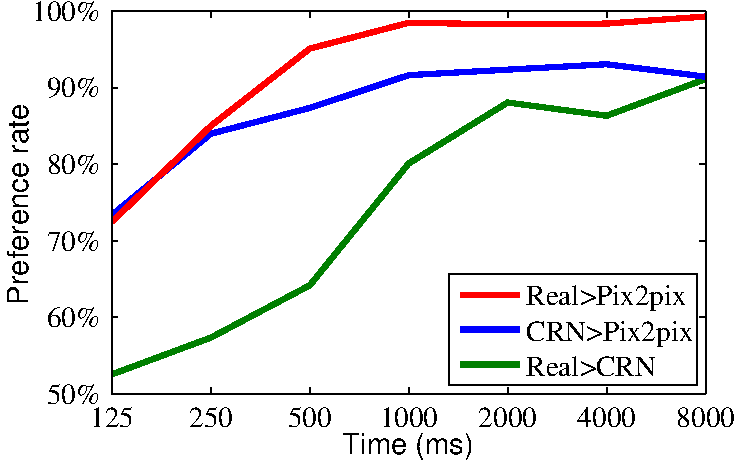
\includegraphics[width=0.95\linewidth]{figures/cityscapes_plot6.pdf}
\caption{Time-limited pairwise comparisons on Cityscapes.}
\label{fig:cityscapes-timed}
\vspace{-1mm}
\end{figure}


\begin{figure*}[t]
\centering
\begin{tabular}{@{}c@{\hspace{0.8mm}}c@{\hspace{0.8mm}}c@{}}

\includegraphics[width=0.33\linewidth]{figures/qualitative/label.png}&
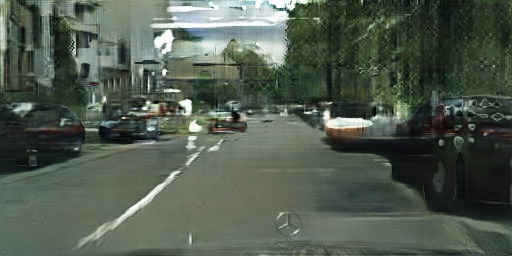
\includegraphics[width=0.33\linewidth]{figures/qualitative/GAN.jpg}&
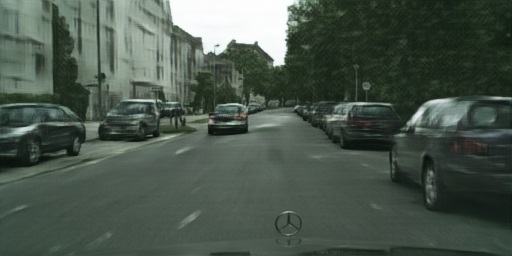
\includegraphics[width=0.33\textwidth]{figures/qualitative/dilated.jpg}\vspace{-1mm}\\
\small Semantic layout & \small GAN+semantic segmenation & \small Full-resolution network  \vspace{1mm}\\

\includegraphics[width=0.33\linewidth]{figures/qualitative/ours.jpg}&

\includegraphics[width=0.33\textwidth]{figures/qualitative/pix2pix.jpg}&
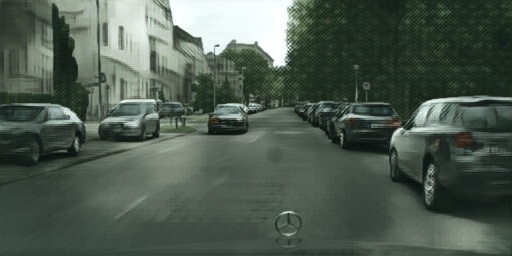
\includegraphics[width=0.33\linewidth]{figures/qualitative/unet.jpg}\vspace{-1mm}\\
\small Our result & \small Isola et al.~\cite{Isola2017} & \small Encoder-decoder \vspace{1mm}\\
\end{tabular}
\caption{Qualitative comparison on the Cityscapes dataset.}
\label{fig:visual_cityscapes}
%\end{figure*}
\vspace{3mm}

%\begin{figure*}[t]
\centering
\begin{tabular}{@{}c@{\hspace{0.3mm}}c@{\hspace{0.3mm}}c@{\hspace{0.3mm}}c@{\hspace{0.3mm}}c@{}}
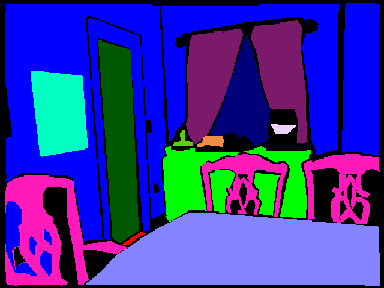
\includegraphics[width=0.198\linewidth]{figures/NYU/label1.png}&
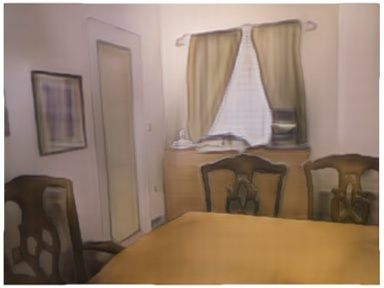
\includegraphics[width=0.198\linewidth]{figures/NYU/ours1b.jpg}&
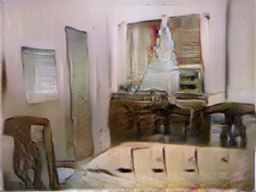
\includegraphics[width=0.198\linewidth]{figures/NYU/pix2pix1.jpg}&
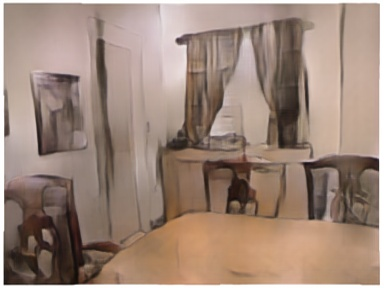
\includegraphics[width=0.198\linewidth]{figures/NYU/dilated1.jpg}&
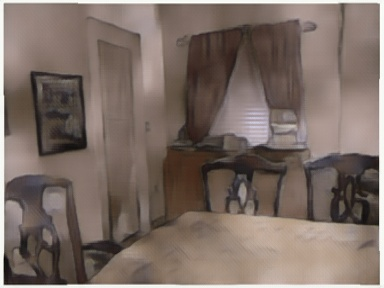
\includegraphics[width=0.198\linewidth]{figures/NYU/unet1.jpg}\\
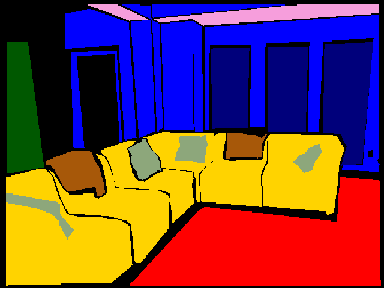
\includegraphics[width=0.198\linewidth]{figures/NYU/label2.png}&
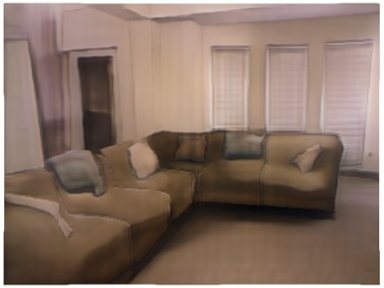
\includegraphics[width=0.198\linewidth]{figures/NYU/ours2b.jpg}&
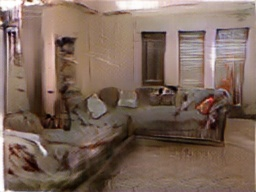
\includegraphics[width=0.198\linewidth]{figures/NYU/pix2pix2.jpg}&
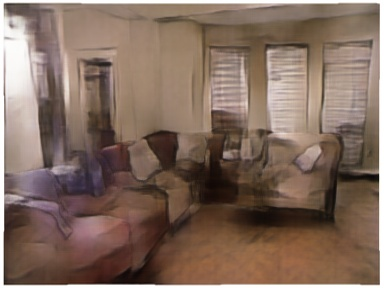
\includegraphics[width=0.198\linewidth]{figures/NYU/dilated2.jpg}&
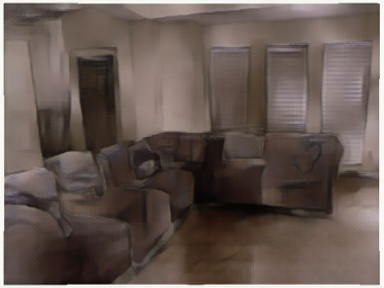
\includegraphics[width=0.198\linewidth]{figures/NYU/unet2.jpg}\\
\small Semantic layout & \small Our result & \small Isola et al.~\cite{Isola2017} & \small Full-resolution network & \small Encoder-decoder \vspace{1mm}\\
\end{tabular}
\caption{Qualitative comparison on the NYU dataset.}
\label{fig:visual_nyu}
%\end{figure*}
\vspace{3mm}

%\begin{figure*}[t]
\centering
\begin{tabular}{@{}c@{\hspace{0mm}}c@{\hspace{0mm}}c@{\hspace{0mm}}c@{}}
%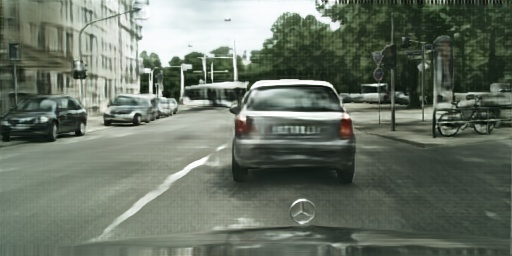
\includegraphics[height=3.25cm]{figures/diversity/cityscapes3b.jpg}&
%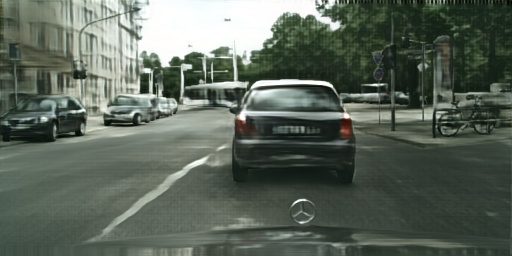
\includegraphics[height=3.25cm]{figures/diversity/cityscapes4c.jpg}&
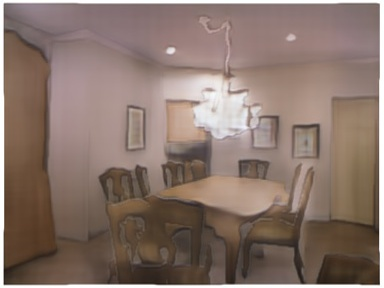
\includegraphics[height=3.25cm]{figures/diversity/nyu3b.jpg}&
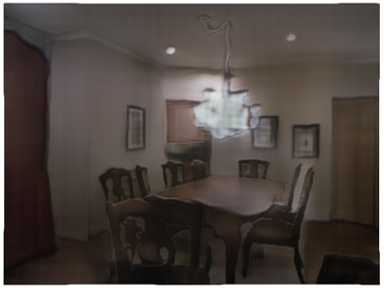
\includegraphics[height=3.25cm]{figures/diversity/nyu4b.jpg}&
%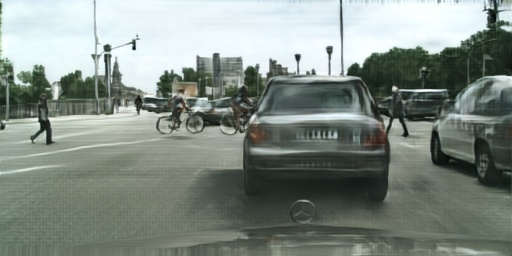
\includegraphics[height=3.25cm]{figures/diversity/cityscapes1.jpg}&
%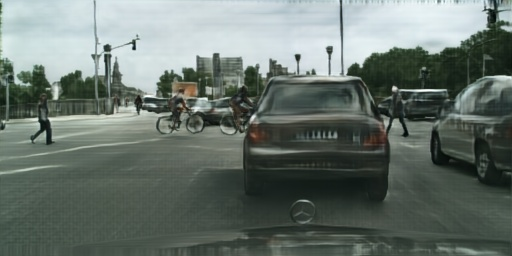
\includegraphics[height=3.25cm]{figures/diversity/cityscapes2.jpg}&
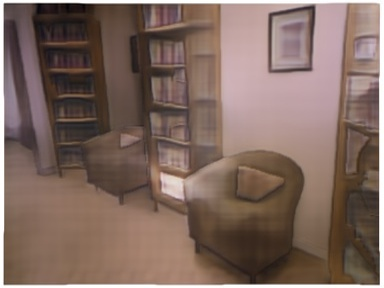
\includegraphics[height=3.25cm]{figures/diversity/nyu1b.jpg}&
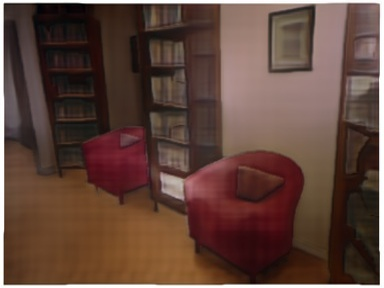
\includegraphics[height=3.25cm]{figures/diversity/nyu2b.jpg}\\
\end{tabular}
\caption{Synthesizing a diverse collection, illustrated on the NYU dataset. Each pair shows two images from a collection synthesized for a given semantic layout.
%Results on the Cityscapes dataset on the left, results on the NYU dataset on the right. For each dataset, each row shows two of the images in the synthesized collection.
}
\label{fig:diversity}
%\vspace{-3mm}
\vspace{-2mm}
\end{figure*}


At 250 milliseconds ($\frac{1}{4}$ of a second), the Real$>$Pix2pix rate rises to 85.0\% while the Real$>$CRN rate is at 57.4\%. The CRN$>$Pix2pix rate is 84.0\%, still nearly identical to Real$>$Pix2pix. At 500 milliseconds, the Real$>$Pix2pix and CRN$>$Pix2pix rates finally diverge, although both are extremely high (95.1\% and 87.4\%, respectively), and the Real$>$CRN rate rises to 64.2\%. Over time, the CRN$>$Pix2pix rate rises above 90\% and the Real$>$Pix2pix rate remains consistently higher than the Real$>$CRN rate.

\mypara{NYU dataset.}
We conduct supporting experiments on the NYU dataset. This dataset is smaller and lower-resolution, so the quality of images synthesized by all approaches is lower. Nevertheless, the differences are still clear. Table~\ref{table:cityscapes} reports the results of randomized pairwise comparisons of images synthesized for this dataset. Images synthesized by the presented approach were again rated consistently more realistic than the baselines. All results are statistically significant with $p < 10^{-3}$. Qualitative results are shown in Figure~\ref{fig:visual_nyu}.
%Compared to the approach of Isola et al.~\cite{Isola2017}, images synthesized by the CRN were rated more realistic in 97\% of the comparisons.

%Quantitative results on the GTA5 dataset and the NYU dataset are reported in the supplement. We have also used models trained on Cityscapes to synthesize images for GTA5 semantic layouts. The results are consistent with the results on the Cityscapes dataset.

\begin{comment}
\begin{table}[h]
   \centering
  \begin{tabular}{@{}l@{\hspace{3mm}}c@{\hspace{3mm}}c@{\hspace{3mm}}c@{}}
     \toprule
    & {\small Image-space} & \small{Isola et al.~\cite{Isola2017}} & \small{Full-resolution}\\       \midrule
   {\small Ours $>$ Baseline}&   \bfseries \small 91.4\% &  \bfseries \small 77.2\% &  \bfseries \small 65.8\% \\
   {\small Baseline $>$ Ours}&   8.6\% &  \small 22.8\% &  \small 34.2\% \vspace{0.5mm}\\
%   {\small GTA5} &  \% & "50.3"\% & \% \\
%   {\small Cityscapes$\rightarrow$GTA5} &  "97"\%& 75.2\% & 55.4\% \\
 \bottomrule
\end{tabular}
\caption{Results of pairwise comparisons of images synthesized by models trained on the NYU dataset.}
\label{table:nyu}
%\vspace{0.5mm}
\vspace{-0.5mm}
\end{table}
\end{comment}

\mypara{Diversity loss.}
%Figure~\ref{fig:visual_cityscapes} shows a qualitative comparison of models trained on the Cityscapes dataset.
For all preceding experiments we have used the feature matching loss specified in Equation~\ref{eq:loss}. The models produced a single image as output, and this image was evaluated against baselines. We now qualitatively demonstrate the effect of the diversity loss described in Section~\ref{sec:diversity}. To this end we trained models that produce image collections as output (9 images at a time). Figure~\ref{fig:diversity} shows pairs of images sampled from the synthesized collections, for different input layouts in the NYU validation set. The figure illustrates that the diversity loss does lead the output channels to spread out and produce different appearances.
%Figure~\ref{fig:diversity} shows the effect of the diversity loss described in Section~\ref{sec:diversity}. We use $k=9$ in all experiments. Figure~\ref{fig:diversity} visualizes the output of 2 out of the $k$ output 3-tuples. The same 3-tuples are used for each row, showing that the diversity loss causes output channels to specialize: after training, some channels begin to specialize in black cars, others in white cars, etc. This illustrates that the diversity loss successfully enables the outputs to diversify and cover the space of object appearances.

%\mypara{Additional results.}
%Additional results are presented in the supplement.


\begin{comment}

MATERIAL FOR THE SUPPLEMENT:

      \mypara{Comparison on Cityscapes.}
      We compare our CRN model to the four baselines on the Cityscapes dataset. All the models are trained on the Cityscapes training set and generate 500 output images on the semantic layouts in the  validation set. We construct four batches of HITs and each batch is for comparisons between our model and a baseline. In each batch, we have 5 HITS each containing 110 comparisons. In each HIT, there are 100 "our vs baseline" comparisons. The other 10 comparisons are sentinel comparisons where a real cityscape image is compared to a synthesized image. For each comparison, two images are displayed in a row and the user is required to pick an image which is more realistic.

      We make sure that each of the 500 comparisons appear exactly once in a batch. The order of two images for each comparison is randomized. The order of all the comparisons are also randomized. Each HIT is given 15 minutes to complete and is completed by 10 workers. There are 50 unique workers for each batch. We discard the submissions of a worker who fails twice or more on sentinel comparisons. We pay 1 dollar to each worker who completes a HIT.

      Table \ref{table:cityscapes} summarizes the results which suggest that our CRN model outperforms all the baselines.

      \mypara{Timed comparison on Cityspaces.}
      Here, we consider pairwise comparisons among our CRN model, real Cityscapes images, and Image-to-image model. Given enough time, humans are able to tell the real image is more realistic than synthesized images. Therefore, we are interested how quickly a person can tell the real image is more realisitc. We add time constraints for comparison. In each comparison, two images are shown simultaneously for some amount of time and then disappear. We choose $\frac{1}{8}$, $\frac{1}{4}$, $\frac{1}{2}$, 1, 2, 4, and 8 seconds as time periods in this experiment. Since we have three types of pairwise comparisons: "Ours vs Cityscapes", "Image-to-image vs Cityscapes" and "Ours vs Image-to-image", there are $3\times 7=21$ modes in this experiment.

      We totally construct 10 HITs each having 110 comparisons. In each HIT, we have 105 pairwise comparisons for the 21 modes so that each mode has 5 comparisons. 5 sentinel comparisons are added: "Cityscapes vs image-space loss" with 4 seconds. The submissions of a worker are discard if the worker fails any sentinel comparison. For each comparison, we randomly choose one semantic layout in Cityscapes validation for comparison. The order of the two images in a comparison is randomized as well as the order of the comparisons. Each HIT is completed by 10 workers and we have totally 100 unique workers in this experiment. We pay 2 dollars to each worker who completes a HIT.

      Figure \ref{fig:time_cityscapes} shows the experiment results. The results show that humans could not differentiate our synthesized image and real images in less than $\frac{1}{2}$ second, but can differentiate synthesized images by Image-to-image and the real images in just $\frac{1}{8}$ seconds.

      \mypara{Timed comparison on GTA5 layouts.}
      Here we test the cross-dataset generalization. We consider pairwise comparisons among our CRN model, Image-to-image and the GTA images. We use the same experiment setup for timed comparison on Cityscapes, except that we use "Cityscapes vs GAN+semantic segmenation" as sentinel comparisons (for more diverse comparisons in overall experiments).

      The result is illustrated in Figure \ref{fig:timed_GTA5}. Our model demonstrates strong cross-dataset generalization, even though the model is never trained on GTA semantic layouts.

      \begin{figure}[h]
      \centering
      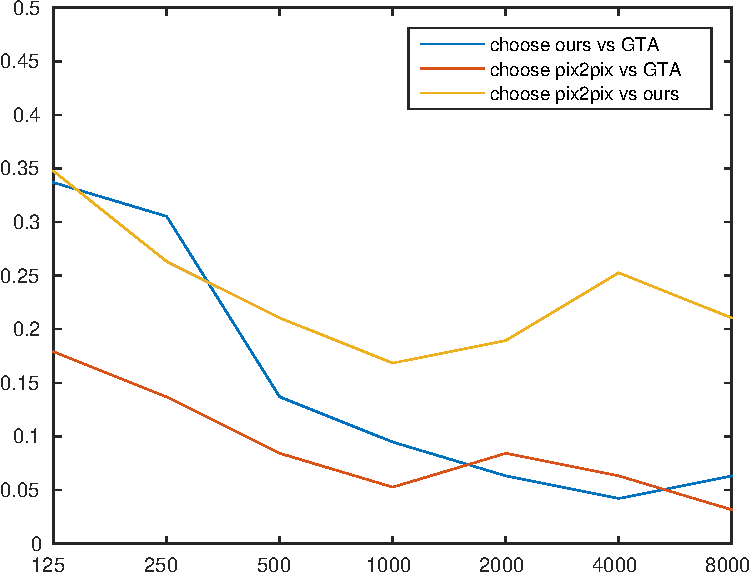
\includegraphics[width=0.35\textwidth]{figures/GTA5_plot.pdf}
      \caption{Placeholder. Comparison with time limitation per pair on GTA5. Only 19\% data are collected, so the result is not stable. CONTENT will be updated today.}
      \label{fig:timed_GTA5}
      \end{figure}


      \mypara{Comparison on NYU.}
      We compare our model with the other two baselines, image-space loss and Image-to-Image model. Our result is summarized in Table \ref{table:NYU_comparison}.

      \begin{table}[h]
         \centering
        \setlength{\tabcolsep}{3.3mm}
         \ra{1.1}
        \begin{tabular}{@{}c@{\hspace{10mm}}cc@{}}
           \toprule
          Method  &   Image-to-Image  & Image space loss\\       \midrule
         Our preference&    & \\
         Our disfavor &  & \\
         p-value &  &  \\
       \bottomrule
      \end{tabular}
      \caption{Comparison on NYU.}
      \label{table:NYU_comparison}
      \end{table}

      \mypara{Visual comparison on Cityscapes.}
      We compare our approach to other baselines visually in Figure \ref{fig:visual_cityscapes}.

      \mypara{Visual comparison on GTA.}
      We compare our approach to other baselines visually in Figure \ref{fig:visual_GTA}.

      \mypara{Visual comparison on NYU.}
      We compare our approach to other two baselines visually in Figure \ref{fig:visual_NYU}.

      \mypara{Stress test.}
      Our results with a coarse semantic layout is demonstrated in Figure \ref{fig:coarse}.

      \begin{figure*}
      \centering
      \begin{tabular}{@{}c@{\hspace{0.8mm}}c@{\hspace{0.8mm}}c@{}}
      
\includegraphics[width=0.33\linewidth]{figures/NYU/L1.jpg}&
      
\includegraphics[width=0.33\linewidth]{figures/NYU/ours.jpg}&
      
\includegraphics[width=0.33\textwidth]{figures/NYU/pix2pix.jpg}\\
      Image-space loss & Ours & Image-to-image\\
      \end{tabular}
      \caption{Visual comparison on GTA.}
      \label{fig:visual_GTA}
      \end{figure*}


      \begin{figure}
      \centering
      \begin{tabular}{@{}c@{\hspace{0.8mm}}c@{}}
      
\includegraphics[width=0.49\linewidth]{figures/coarse/label.png}&
      
\includegraphics[width=0.49\linewidth]{figures/coarse/ours.jpg}\\
      Coarse layout & Ours \\
      \end{tabular}
      \caption{Coarse semantic layout.}
      \label{fig:coarse}
      \end{figure}

\end{comment}
